\documentclass[6008notes.tex]{subfiles}
\begin{document}
\graphicspath{ {images/hiddenmarkov/} }

\section{Special Case: Marginalization in Hidden Markov Models}

\subsection{Introduction to Hidden Markov Models (HMM's)}

We now show the sum-product algorithm applied to the special case of a tree-structured graphical model called a hidden Markov model (HMM), for which we have hidden states $X_{1},X_{2},\dots ,X_{n}$ that we infer given observations $Y_{1},Y_{2},\dots ,Y_{n}$, and the graphical model looks as follows:

{\centering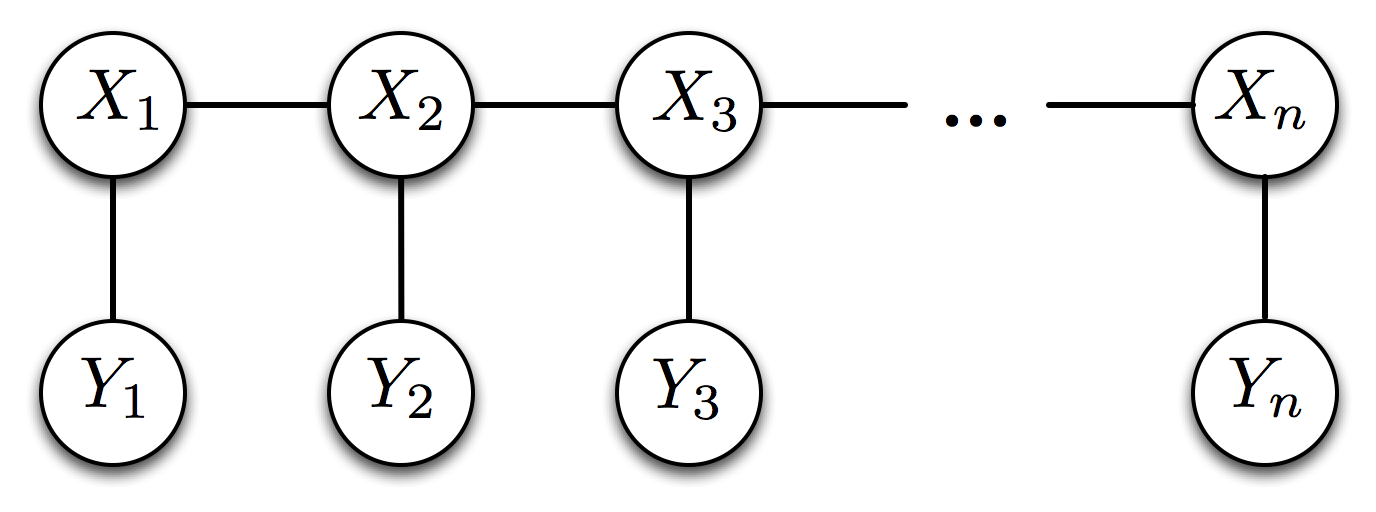
\includegraphics[scale=0.4]{images_sec-graphical-models-hmm} \par}

For example, in a basic robot localization problem setup, $X_i$ is the robot's location at time point $i$, and $Y_i$ is the robot's sensor readings at time point $i$. Then $p_{X_{i}\mid Y_{1},\dots ,Y_{n}}(\cdot \mid y_{1},\dots ,y_{n})$ is the posterior distribution of the robot's location at time point i.

The graphical model is

{\centering{\renewcommand{\arraystretch}{1.5}
\begin{tabular}{l l l}
& $p_{X_{1},\dots ,X_{n},Y_{1},\dots ,Y_{n}}(x_{1},\dots ,x_{n},y_{1},\dots ,y_{n})$ & \\
& $\propto \prod _{i=1}^{n}\big \{ \phi _{X_{i}}(x_{i})\phi _{Y_{i}}(y_{i})\psi _{X_{i},Y_{i}}(x_{i},y_{i})\big \} \prod _{i=1}^{n-1}\psi _{X_{i},X_{i+1}}(x_{i},x_{i+1}).$ &
\end{tabular}} \par}

Note that by incorporating observations, we are left with a new graphical model that is only over the $X_i$'s:

{\centering{\renewcommand{\arraystretch}{1.5}
\begin{tabular}{l l l}
&  $p_{X_{1},\dots ,X_{n}\mid Y_{1},\dots ,Y_{n}}(x_{1},\dots ,x_{n}\mid y_{1},\dots ,y_{n})$ & \\
&  $\propto \prod _{i=1}^{n}\big \{ \underbrace{\phi _{X_{i}}(x_{i})\phi _{Y_{i}}(y_{i})\psi _{X_{i},Y_{i}}(x_{i},y_{i})}_{\triangleq \widetilde{\phi }_{i}(x_{i})}\big \} \prod _{i=1}^{n-1}\underbrace{\psi _{X_{i},X_{i+1}}(x_{i},x_{i+1})}_{\triangleq \psi _{i,i+1}(x_{i},x_{i+1})}.$ & 
\end{tabular}} \par}

{\centering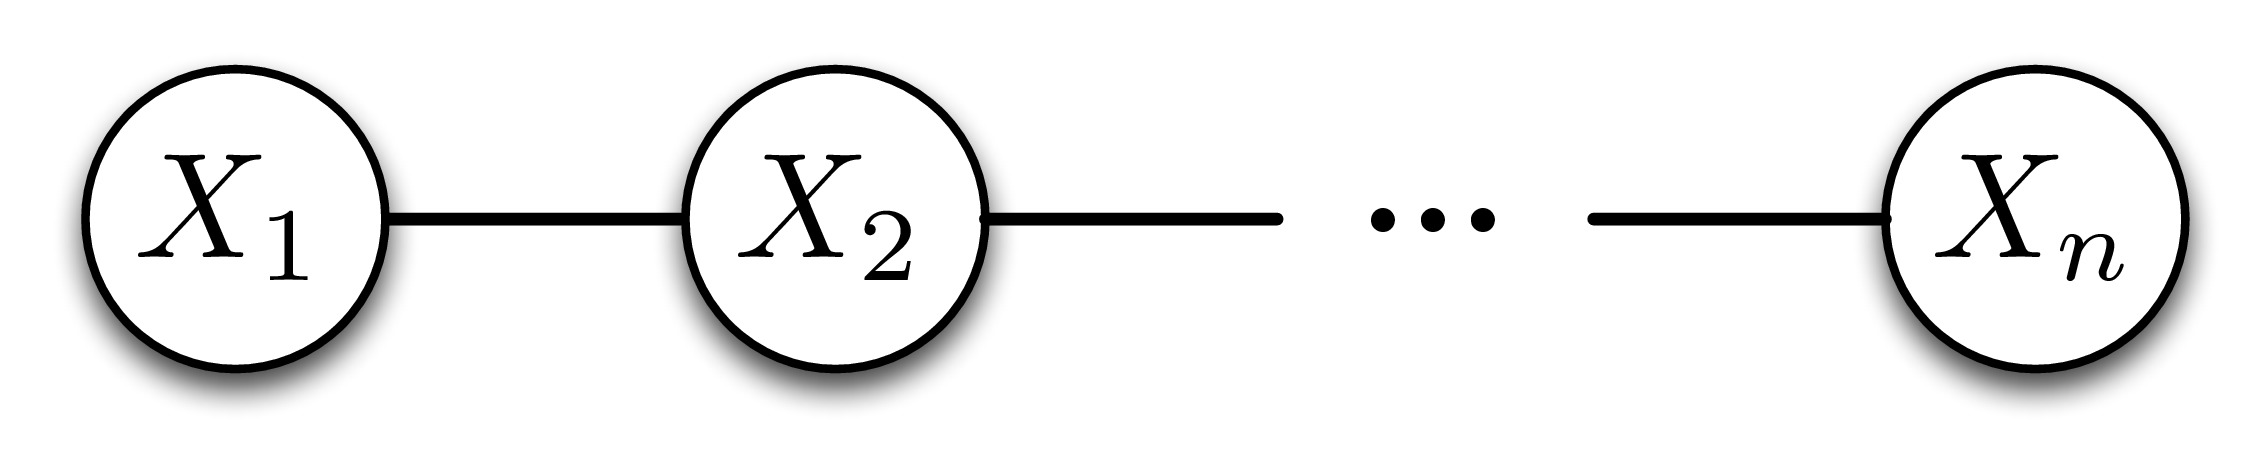
\includegraphics[scale=0.4]{images_sec-graphical-models-markov-chain} \par}

We can run the sum-product algorithm choosing the right-most node $X_n$ as the root, so the initial message passing happens from the single leaf node $X_1$ going rightward until reaching $X_n$ (this is called the forward pass), and then we pass messages from the root node $X_n$ all the way back to $X_1$ (this is called the backward pass). The resulting algorithm for this specific case of HMM's is called the forward-backward algorithm.

Hidden Markov models are widely used in practice for more than just robot localization (note that a robot could be, for instance, a self-driving car)! But a few other examples include recognizing speech, labeling the part of speech of each word in a sentence, aligning DNA sequences, detecting protein folds, and decoding a certain of code in digital communications called a convolutional code.


\subsection{Hidden Markov Models: Three Ingredients}

Often for HMM's, a problem is modeled with a prior distribution $p_{X_1}$ on the initial state $X_1$, a transition model $p_{X_{i+1}\mid X_{i}}$ that is the same for all $i$ (so we can denote it as just $p_{X_{\text {next}}\mid X_{\text {current}}}$), and an observation model $p_{Y_{i}\mid X_{i}}$ that is the same for all $i$ (so we can denote it as just $p_{Y\mid X}$), in which case

{\centering{\renewcommand{\arraystretch}{1.5}
\begin{tabular}{l l l}
 & $p_{X_{1},\dots ,X_{n},Y_{1},\dots ,Y_{n}}(x_{1},\dots ,x_{n},y_{1},\dots ,y_{n})$ & \\
 & $=p_{X_{1}}(x_{1})\bigg\{ \prod _{i=1}^{n}p_{Y\mid X}(y_{i}\mid x_{i})\bigg\} \bigg\{ \prod _{i=1}^{n-1}p_{X_{\text {next}}\mid X_{\text {current}}}(x_{i+1}\mid x_{i})\bigg\} .$ & 
\end{tabular}} \par}

Then as a graphical model, incorporating observations $Y_{1}=y_{1},\dots ,Y_{n}=y_{n}$,

{\centering{\renewcommand{\arraystretch}{1.5}
\begin{tabular}{l l l}
 & $$ & \\
 & $$ & 
\end{tabular}} \par}

The messages are:

{\centering{\renewcommand{\arraystretch}{1.5}
\begin{tabular}{r c l}
$m_{1\rightarrow 2}(x_{2})$ & $=$ & $\sum _{x_{1}}\widetilde{\phi }_{1}(x_{1})\psi _{1,2}(x_{1},x_{2})$ \\
$\displaystyle \text {For }i=2,\dots ,n-1:\qquad m_{i\rightarrow i+1}(x_{i+1})$ & $=$ & $\sum _{x_{i}}\widetilde{\phi }_{i}(x_{i})\psi _{i,i+1}(x_{i},x_{i+1})m_{i-1\rightarrow i}(x_{i})$ \\ 
$\displaystyle m_{n\rightarrow n-1}(x_{n-1})$ & $=$ & $\sum _{x_{n}}\widetilde{\phi }_{n}(x_{n})\psi _{n-1,n}(x_{n-1},x_{n})$ \\
$\displaystyle \text {For }i=2,\dots ,n-1:\qquad m_{i\rightarrow i-1}$ & $=$ & $\sum _{x_{i}}\widetilde{\phi }_{i}(x_{i})\psi _{i-1,i}(x_{i-1},x_{i})m_{i+1\rightarrow i}(x_{i})$ 
\end{tabular}} \par}

The posterior distributions for each $X_i$ given all the observations $Y_{1}=y_{1},\dots ,Y_{n}=y_{n}$ are:

{\centering{\renewcommand{\arraystretch}{1.5}
\begin{tabular}{r c l}
$p_{X_{1}\mid Y_{1},\dots ,Y_{n}}(x_{1}\mid y_{1},\dots ,y_{n})$ & $\propto$ & $\widetilde{\phi }_{1}(x_{1})m_{2\rightarrow 1}(x_{1})$ \\
$\displaystyle \text {For }i=2,\dots ,n-1:\qquad p_{X_{i}\mid Y_{1},\dots ,Y_{n}}(x_{1}\mid y_{1},\dots ,y_{n})$ & $\propto$ & $\widetilde{\phi }_{i}(x_{i})m_{i-1\rightarrow i}(x_{i})m_{i+1\rightarrow i}(x_{i})$ \\ 
$\displaystyle p_{X_{n}\mid Y_{1},\dots ,Y_{n}}(x_{1}\mid y_{1},\dots ,y_{n})$ & $\propto$ & $\widetilde{\phi }_{n}(x_{n})m_{n-1\rightarrow n}(x_{n})$ 
\end{tabular}} \par}

We will use these conventions:

\begin{itemize}
\item The forward messages are denoted by $\alpha _{i\rightarrow i+1}(x_{i+1})\triangleq m_{i\rightarrow i+1}(x_{i+1})$

\item The backward messages are denoted by $\beta _{i+1\rightarrow i}(x_{i})\triangleq m_{i+1\rightarrow i}(x_{i})$

\item Since $\psi _{i,i+1}$ is actually the same table/function for all $i$, we just call it $\psi$, i.e., $\psi (x_{i},x_{i+1})=p_{X_{\text {next}}\mid X_{\text {current}}}(x_{i+1}\mid x_{i})$

\item Since $\widetilde{\phi}_{i}$ above is actually the same for all $i \ge 2$, we just call it $\widetilde{\phi}$, i.e., $\psi (x_{i},x_{i+1})=p_{X_{\text {next}}\mid X_{\text {current}}}(x_{i+1}\mid x_{i})$; we actually extend this to the case $i=1$ as well with the following notational convenience: we define $\alpha _{0\rightarrow 1}(x_{1})\triangleq p_{X_{1}}(x_{1})$, so that the forward messages now can be expressed in 1 formula:

{\centering$\alpha _{i\rightarrow i+1}(x_{i+1})=\sum _{x_{i}}\widetilde{\phi }(x_{i})\psi (x_{i},x_{i+1})\alpha _{i-1\rightarrow i}(x_{i})\qquad \text {for all }i=1,2,\dots ,n-1$ \par}
 
\item As another notational convenience, we define $\beta _{n+1\rightarrow n}(x_{n})=1$ for all $x_n$, so that the backward messages now can be expressed in one formula:

{\centering$\beta _{i\rightarrow i-1}=\sum _{x_{i}}\widetilde{\phi }(x_{i})\psi (x_{i-1},x_{i})\beta _{i+1\rightarrow i}(x_{i})\qquad \text {for all }i=2,3,\dots ,n$ \par}

\end{itemize}
 
\paragraph{Clarification:} In terms of edges in the graphical model, any particular state variable $X_k$ has edges only to $X_{k-1}$ (what came before it), $X_{k+1}$ (what comes after it), and $Y_k$ (the observation associated with it). When we condition on all three of these, $X_k$ becomes independent of everything else in the graph. \textit{However, when we don't condition on anything, then from any node we can reach any other node, so at least from looking at the graph, it could very well be that nodes far apart depend on each other. Even if we condition on all the $Y_i$'s and nothing else, in general, all the $X_i$'s can be related to each other!}

As a reminder, here is the graphical model for an HMM:

{\centering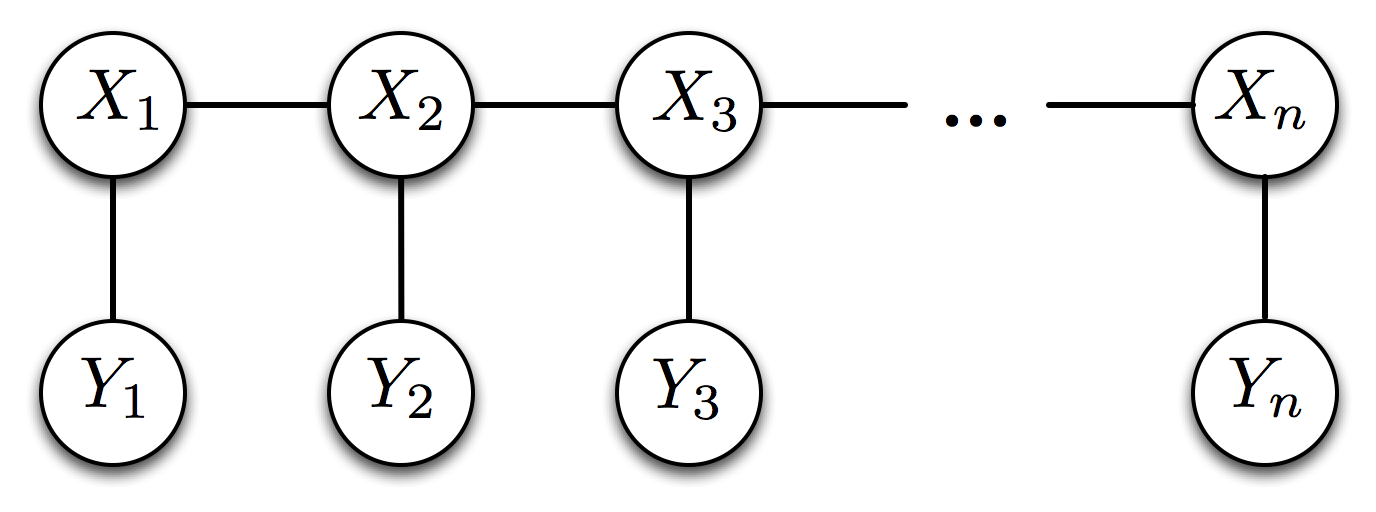
\includegraphics[scale=0.4]{images_sec-graphical-models-hmm} \par}

Here's a quick recap of the important facts:

\begin{itemize}
\item We observe $Y_1$ through $Y_n$, which we model as coming from hidden states $X_1$ through $X_n$

\item The goal of the forward-backward algorithm is to find the conditional distribution over hidden states given the data.

\item In order to specify an HMM, we need three quantities:

\begin{itemize}
\item A \textit{transition distribution}, $p_{X_{k+1}|X_ k}(x_{k+1}|x_ k)$, which describes the distribution for the next state given the current state. This is often represented as a matrix that we'll call $A$. Rows of $A$ correspond to the current state, columns correspond to the next state, and each entry corresponds to the transition probability. That is, the entry at row $i$ and column $j$, $A_{ij}$, is $p_{X_{k+1}|X_ k}(j|i)$.

\item An \textit{observation distribution} (also called an ``emission distribution'') $p_{Y_ k|X_ k}(y_ k|x_ k)$, which describes the distribution for the output given the current state. We'll represent this with matrix $B$. Here, rows correspond to the current state, and columns correspond to the observation. So, $B_{ij} = p_{Y_ k|X_ k}(j|i)$: the probability of observing output $j$ from state $i$ is $B_{ij}$. Since the number of possible observations isn't necessarily the same as the number of possible states, $B$ won't necessarily be square.

\item An \textit{initial state distribution} $p_{X_1}(x_1)$, which describes the starting distribution over states. We'll represent this with a vector called $\pi_0$, where item $i$ in the vector represents $p_{X_1}(i)$.
\end{itemize}

\item We compute forward and backwards messages as follows:

{\centering{\renewcommand{\arraystretch}{1.5}
\begin{tabular}{r c l}
$\alpha _{(k-1)\to k}(x_{k})$ & $=$ & $\sum _{x_{k-1}} \overbrace{\alpha _{(k-2)\to (k-1)}(x_{k-1})}^{\text {previous message}} \overbrace{\tilde{\phi }(x_{k-1})}^{\text {obs.}} \overbrace{\psi (x_{k-1}, x_{k})}^{\text {transition}}$ \\
$\displaystyle \beta _{(k+1)\to k}(x_{k})$ & $=$ & $\sum _{x_{k+1}} \underbrace{\beta _{(k+2)\to (k+1)}(x_{k+1})}_{\text {previous message}} \underbrace{\tilde{\phi }(x_{k+1})}_{\text {obs.}} \underbrace{\psi (x_{k}, x_{k+1})}_{\text {transition}}$ 
\end{tabular}} \par}

These messages are illustrated below:

{\centering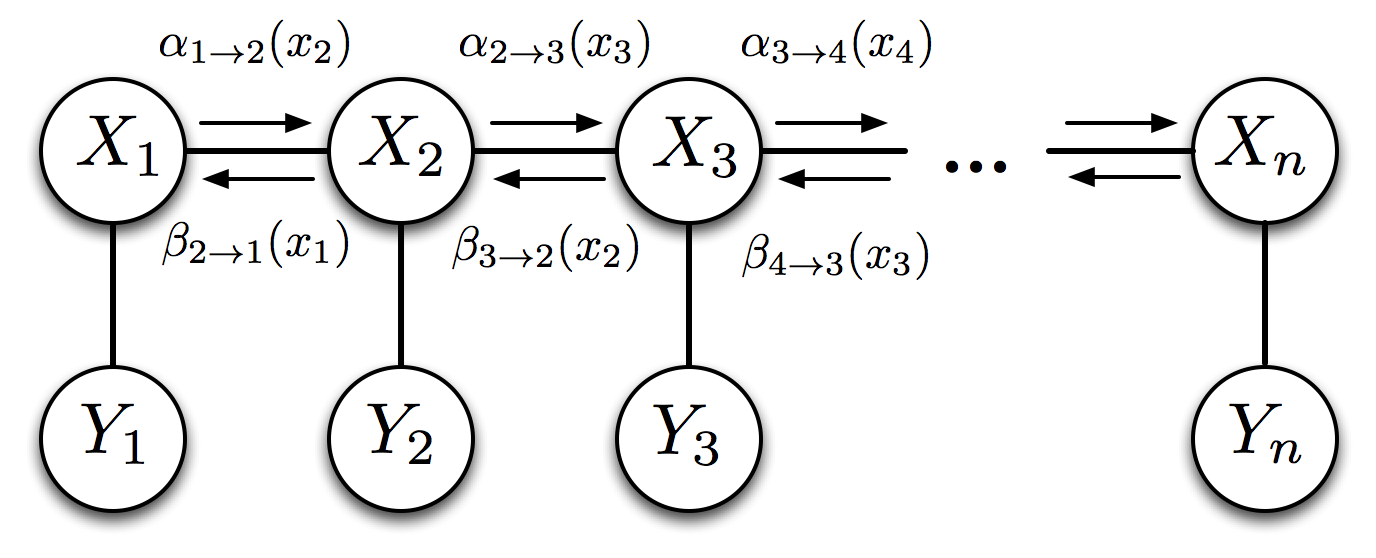
\includegraphics[scale=0.4]{images_sec-graphical-models-hmm-messages} \par}

Here, $\tilde{\phi }(x_ k) = p_{Y_ k|X_ k}(y_ k|x_ k)$ and $\psi (x_ k, x_{k+1}) = p_{X_{k+1}|X_ k}(x_ k|x_{k+1})$. The first forward message $\alpha _{0 \to 1}(x_1)$ is initialized to $\pi _0(x_1) = p_{X_1}(x_1)$. The first backward message $\beta _{(n+1)\to n}(x_ n)$ is initialized to uniform (this is equivalent to not including it at all).

The picture below illustrates the computation of one forward message $\alpha _{2 \to 3}(x_3)$.

{\centering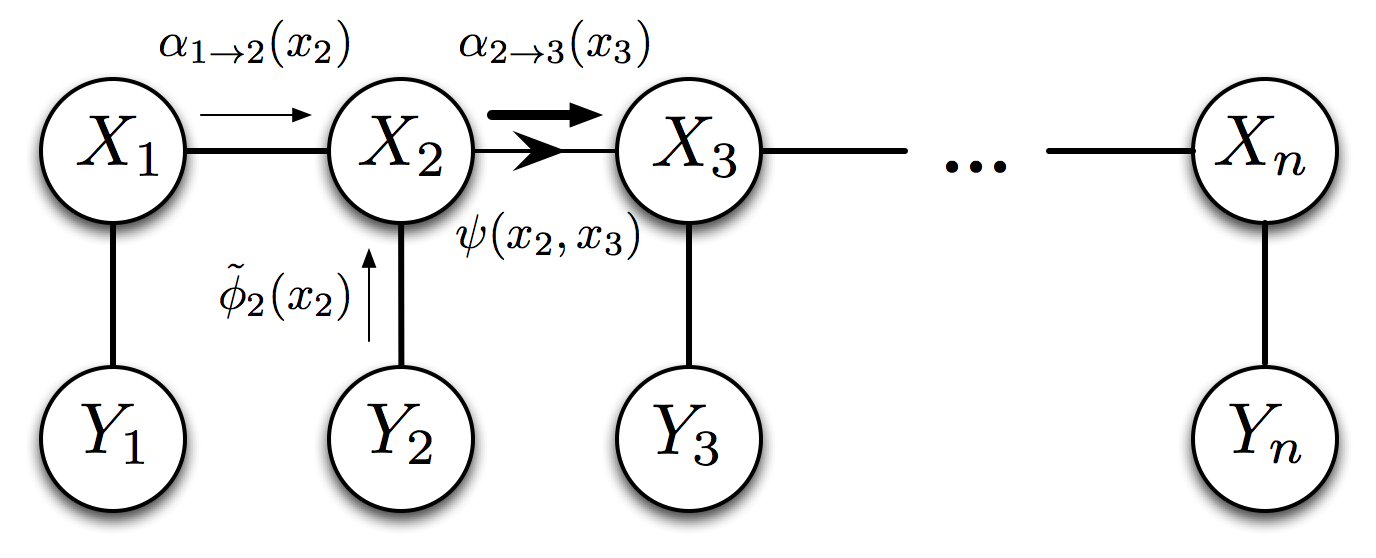
\includegraphics[scale=0.4]{images_sec-graphical-models-hmm-forward-message} \par}

In order for node 2 to summarize its belief about $X_3$, it must incorporate the previous message $\alpha _{1 \to 2}(x_2)$, its observation $\tilde{\phi }(x_2)$, and the relationship $\psi (x_2,x_3)$ between $X_2$ and $X_3$.

\item To obtain a marginal distribution for a particular state given all the observations, $p_{X_ k|Y_1,\ldots ,Y_ n}$, we simply multiply the incoming messages together with the observation term, and then normalize:

{\centering$\alpha _{(k-1)\to k}(x_{k})\beta _{(k+1)\to k}(x_{k}) \tilde{\phi }(x_ k) \quad \propto \quad \alpha _{(k-1)\to k}(x_{k})\beta _{(k+1)\to k}(x_{k}) \tilde{\phi }(x_ k)$ \par}
	 	 
Here, the symbol $\propto$ means ``is proportional to'', and indicates that we must normalize at the end so that the answer sums to 1.
\end{itemize}

\paragraph{Technical note:} Traditionally, the backward messages $\beta$ are computed as described here, but the forward messages $\alpha$ are computed as $\alpha ^\prime _{2 \to 3}(x_3) = \alpha _{2 \to 3}(x_3) \tilde{\phi }(x_3)$. In general, this means that the forward message to $X_k$ would also include the observation $Y_k$. How would you modify the equations we have presented to use messages $\alpha ^\prime _{2 \to 3}(x_3) = \alpha _{2 \to 3}(x_3) \tilde{\phi }(x_3)$ and $\beta$ instead and still produce the correct marginals?


\subsection{Formulating HMM's}

Suppose you send your robot, Inquisition, to Mars. Unfortunately, it gets stuck in a canyon while landing and most of its sensors break. You know the canyon has 3 areas. Areas 1 and 3 are sunny and hot, while Area 2 is cold. You decide to plan a rescue mission for the robot from Area 3, knowing the following things about the robot:

\begin{itemize}
\item Every hour, it tries to move forward by one area (i.e. from Area 1 to Area 2, or Area 2 to Area 3). It succeeds with probability $0.75$ and fails with probability $0.25$. If it fails, it stays where it is. If it is in Area 3, it always stays there (and waits to be rescued).

\item The temperature sensor still works. Every hour, we get a binary reading telling us whether the robot's current environment is hot or cold.

\item We have no idea where the robot initially got stuck.
\end{itemize}

Let's construct an HMM for this problem, which amounts to coming up with the transition matrix $A$, observation matrix $B$, and initial state distribution $\pi_0$.

We'll start with the transition matrix. Remember that each row corresponds to the current state, and each column corresponds to the next state. We'll use 3 states, each corresponding to one area.

\begin{itemize}
\item If the robot is in Area 1, it stays where it is with probability 0.25, moves to Area 2 with probability 0.75, and can't move to Area 3.

\item Similarly, if the robot is in Area 2, it stays where it is with probability 0.25, can't move back to Area 1, and moves to Area 3 with probability 0.75.

\item If the robot is in Area 3, it always stays in Area 3.
\end{itemize}

Each item above gives us one row of A. Putting it all together, we obtain

{\centering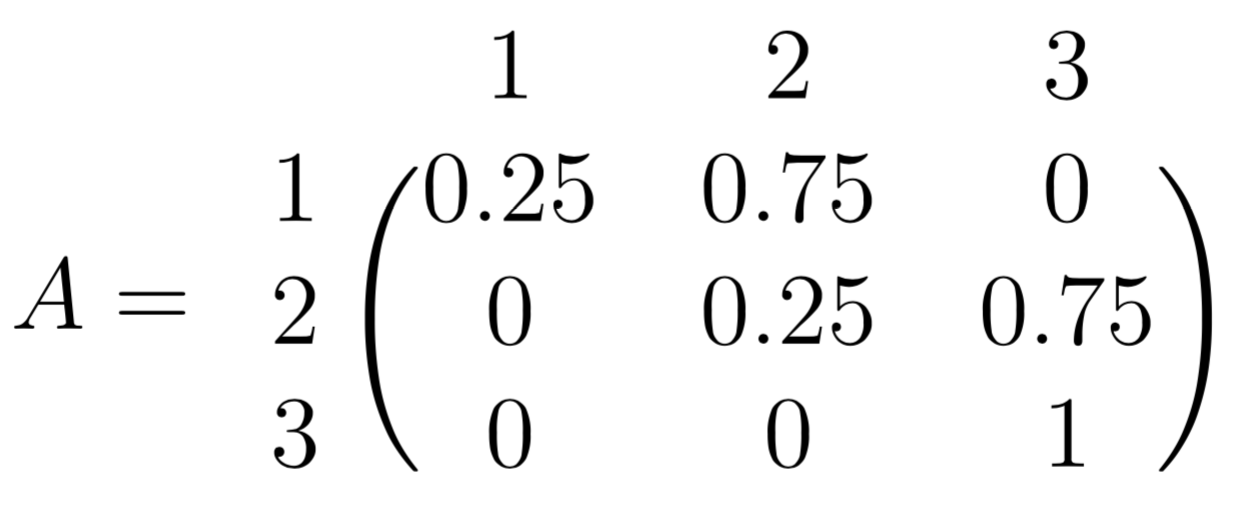
\includegraphics[scale=0.25]{images_sec-formulating-hmm-helper1} \par}

Next, let's look at the observation matrix. There are two possible observations, hot and cold. Areas 1 and 3 always produce ``hot'' readings while Area 2 always produces a ``cold'' reading:

{\centering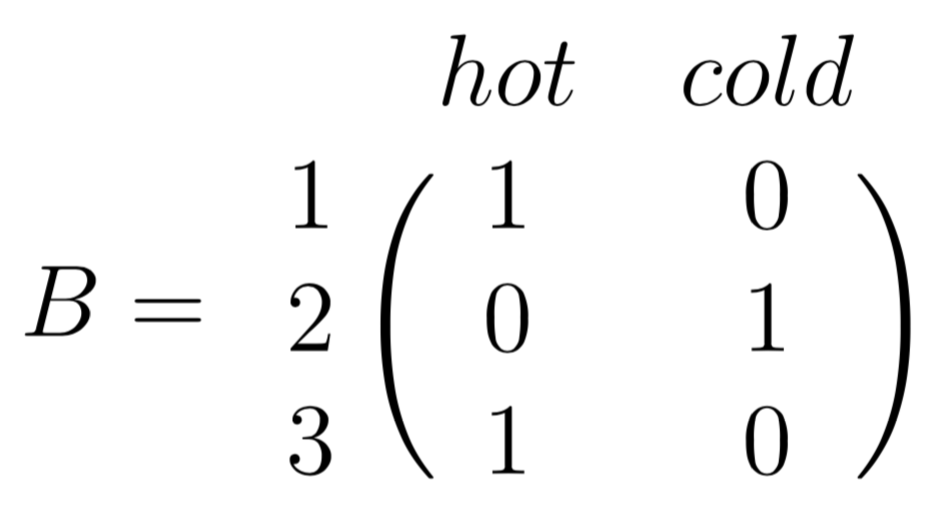
\includegraphics[scale=0.25]{images_sec-formulating-hmm-helper2} \par}

Last but not least, since we have no idea where the robot starts, our initial state distribution will be uniform:

{\centering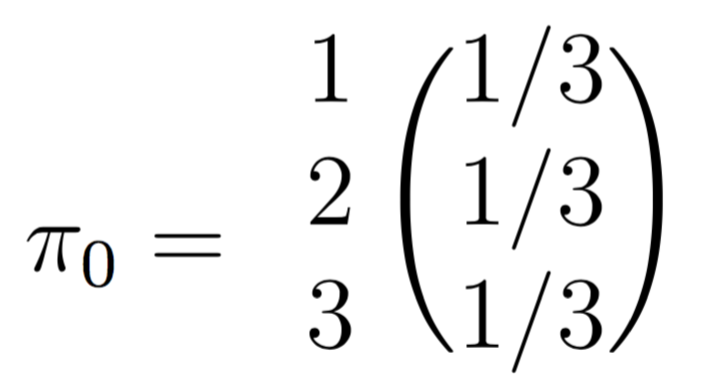
\includegraphics[scale=0.25]{images_sec-formulating-hmm-helper3} \par}


\subsection{Forward and Backward Messages for HMM's}

Before doing any computation, we see that the sequence (hot,cold,hot) could only have been observed from the hidden state sequence (1,2,3). Make sure you convince yourself this is true before continuing!

We'll start with the forward messages.

{\centering$\sum _{x_1} \underbrace{\alpha _{0 \to 1}(x_1) \tilde{\phi }(x_1)}_{\text {depends only on $x_1$}} \psi (x_1,x_2)$ \par}

The output message should have three different possibilities, one for each value of $x_2$. We can therefore represent it as a vector indexed by $x_2$. For each term in the sum (i.e. each possible value of $x_1$):

\begin{itemize}
\item $\alpha _{0 \to 1}$ comes from from the initial distribution. Normally it would come from the previous message, but our first forward message is always set to initial state distribution.

\item $\tilde{\phi }$ comes from the column of $B$ corresponding to our observation $y_1=$ hot.

\item $\psi$ comes from a row of $A$: we are fixing $x_1$ and asking about possible values for $x_1$, which corresponds exactly to the transition distributions given in the rows of $A$ (remember that the rows of $A$ correspond to the current state and the columns correspond to the next state).
\end{itemize}

So, we obtain

\begin{eqnarray*}
		\alpha_{1 \to 2} &= &
		\overbrace{\frac{1}{3} \cdot 1 \cdot \begin{pmatrix} .25 \\ .75 \\ 0 \end{pmatrix}}^{x_1 = 1} +
		\overbrace{\frac{1}{3} \cdot 0 \cdot \begin{pmatrix} 0 \\ .25 \\ .75 \end{pmatrix}}^{x_1 = 2} +
		\overbrace{\frac{1}{3} \cdot 1 \cdot \begin{pmatrix} 0 \\ 0 \\ 1 \end{pmatrix}}^{x_1 = 3} \\
		&\propto& \begin{pmatrix} 1 \\ 3 \\ 4 \end{pmatrix}
\end{eqnarray*}
						
Since our probabilities are eventually computed by multiplying messages and normalizing, we can arbitrary renormalize at any step to make the computation easier.

For the second message, we perform a similar computation:

\begin{eqnarray*}
		\alpha_{2 \to 3} &= &
				\sum_{x_2} {\alpha_{1 \to 2}(x_2) \tilde{\phi}(x_2)} \psi(x_2,x_3) \\
		&= &
				\overbrace{1 \cdot 0 \cdot \begin{pmatrix} .25 \\ .75 \\ 0 \end{pmatrix}}^{x_2 = 1} +
				\overbrace{3 \cdot 1 \cdot \begin{pmatrix} 0 \\ .25 \\ .75 \end{pmatrix}}^{x_2 = 2} +
				\overbrace{4 \cdot 0 \cdot \begin{pmatrix} 0 \\ 0 \\ 1 \end{pmatrix}}^{x_2 = 3} \\
		&\propto& \begin{pmatrix} 0 \\ 1 \\ 3 \end{pmatrix}
\end{eqnarray*}
						
The backwards messages are computed using a similar formula:

\begin{eqnarray*}
                \beta_{3 \to 2} &=& \sum_{x_3} \underbrace{\beta_{4 \to 3}(x_3) \tilde{\phi}(x_3)}_{\text{depends only on $x_3$}} \psi(x_2,x_3)
\end{eqnarray*}
						
The first backwards message, $\beta _{4 \to 3}(x_3)$, is always initialized to uniform since we have no information about what the last state should be. Note that this is equivalent to not including that term at all.

For each value of $x_3$, the transition term $\psi (x_2,x_3)$ is now drawn from a column of $A$, since we are interested in the probability of arriving at $x_3$ from each possible state for $x_2$. We compute the messages as:

\begin{eqnarray*}
		\beta_{3 \to 2} &= &
				\overbrace{1 \cdot \begin{pmatrix} .25 \\ 0 \\ 0 \end{pmatrix}}^{x_3 = 1} +
				\overbrace{0 \cdot \begin{pmatrix} .75 \\ .25 \\ 0 \end{pmatrix}}^{x_3 = 2} +
				\overbrace{1 \cdot \begin{pmatrix} 0 \\ .75 \\ 1 \end{pmatrix}}^{x_3 = 3} \\
		&\propto& \begin{pmatrix} 1 \\ 3 \\ 4 \end{pmatrix}
\end{eqnarray*}

Similarly, the second backwards message is:

\begin{eqnarray*}
		\beta_{2 \to 1} &= &
		\overbrace{1 \cdot 0 \cdot \begin{pmatrix} .25 \\ 0 \\ 0 \end{pmatrix}}^{x_2 = 1} +
		\overbrace{3 \cdot 1 \cdot \begin{pmatrix} .75 \\ .25 \\ 0 \end{pmatrix}}^{x_2 = 2} +
		\overbrace{4 \cdot 0 \cdot \begin{pmatrix} 0 \\ .75 \\ 1 \end{pmatrix}}^{x_2 = 3} \\
		&\propto& \begin{pmatrix} 3 \\ 1 \\ 0 \end{pmatrix}
\end{eqnarray*}

Notice from the symmetry of the problem that our forwards messages and backwards messages were the same.

To compute the marginal distribution for $X_2$ given the data, we multiply the messages and the observation:

\begin{eqnarray*}
		p_{X_2 | Y_1, \ldots, Y_n}(x_2|y_1,\ldots,y_n) &\propto &
				\alpha_{1 \to 2}(x_2)
				\beta_{3 \to 2}(x_2)
				\tilde{\phi}(x_2) \\
		&\propto &
				\begin{pmatrix} 1 \\ 3 \\ 4 \end{pmatrix} \cdot
				\begin{pmatrix} 1 \\ 3 \\ 4 \end{pmatrix} \cdot
				\begin{pmatrix} 0 \\ 1 \\ 0 \end{pmatrix} \\
		&=& \begin{pmatrix} 0 \\ 1 \\ 0 \end{pmatrix} \\
\end{eqnarray*}

Notice that in this case, because of our simplified observation model, the observation ``cold'' allowed us to determine the state. This matches up with our earlier conclusion that the robot must have been in Area 2 during the second hour.


\end{document}
